\chapter{Implementing a NN from Scratch}
\label{sec:nn_from_scratch}

In this Appendix we are going to develop a simple neural network without relying on high-level packages like \texttt{keras} or \texttt{pytorch}.
This is of course a pure exercise to help understanding better how a neural network works, and in production you should always rely on official and well validated \texttt{python} modules.

%Layer by Layer
%We need to keep in mind the big picture here :
%
%We feed input data into the neural network.
%The data flows from layer to layer until we have the output.
%Once we have the output, we can calculate the error which is a scalar.
%Finally we can adjust a given parameter (weight or bias) by subtracting the derivative of the error with respect to the parameter itself.
%We iterate through that process.
%The most important step is the 4th. We want to be able to have as many layers as we want, and of any type. But if we modify/add/remove one layer from the network, the output of the network is going to change, which is going to change the error, which is going to change the derivative of the error with respect to the parameters. We need to be able to compute the derivatives regardless of the network architecture, regardless of the activation functions, regardless of the loss we use.

The goal is to to create a fully connected neural network. In the following Sections we are going to review again each steps of the training focusing on the mathematical aspects needed for the actual implementation.
%convolutional, maxpooling, dropout, etc.) have at least 2 things in common: input ($X$) and output ($Y$) data.

\subsection{Forward Propagation}
In the \emph{forward propagation}, we give the input data to the first layer, then the output of every layer becomes the input of the next until we reach the end of the network. By comparing the result of the network ($Y$) with the desired output (let’s say $\tilde{Y}$), we can calculate an error $E$. The goal is to minimize that error by changing the parameters in the network. That is \emph{backward propagation (backpropagation)}.

\subsection{Gradient Descent}

Basically, we want to change some parameter in the network (call it $w$) so that the total error $E$ decreases. There is a clever way to do it (not randomly) which is the following:

\begin{equation}
	w\leftarrow w - \alpha\cfrac{\partial E}{\partial w}
\end{equation}
where $\alpha$ is a parameter in the range $[0,1]$ that we set and that is called the \emph{learning rate}. 
Anyway, the important thing here is $\frac{\partial E}{\partial w}$. 
We need to be able to find the value of that expression for any parameter of the network regardless of its architecture.

Note that the parameter $\alpha$ should follow an update policy, or an optimizer (e.g. \emph{Adam} in the more complicated examples will see later) , but for the sake of simplicity we’re simply going to keep it constant throughout the entire gradient descent.

\subsection{Backward Propagation}

Suppose that we give a layer the derivative of the error with respect to its output ($\frac{\partial E}{\partial Y}$), then it must be able to provide the derivative of the error with respect to its input ($\frac{\partial E}{\partial X}$).

Remember that $E$ is a scalar and $X$ and $Y$ are matrices.
Let’s forget about $\frac{\partial E}{\partial X}$ for now. The trick here, is that if we have access to $\frac{\partial E}{\partial Y}$ we can very easily calculate $\frac{\partial E}{\partial W}$ (if the layer has any trainable parameters) without knowing anything about the network architecture. We simply use the chain rule:

\begin{equation}
	\cfrac{\partial E}{\partial w} = \sum_i \cfrac{\partial E}{\partial y_j}\cfrac{\partial y_j}{\partial w}
\end{equation}

The unknown is $\frac{\partial y_j}{\partial w}$ which totally depends on how the layer is computing its output. So if every layer have access to $\frac{\partial E}{\partial Y}$ then we can update our parameters.

Don’t forget, the output of one layer is the input of the next layer. Which means $\frac{\partial E}{\partial X}$ for one layer is $\frac{\partial E}{\partial Y}$ for the previous layer. Again, we can use the chain rule:

\begin{equation}
	\cfrac{\partial E}{\partial x_i} = \sum_j \cfrac{\partial E}{\partial y_j}\cfrac{\partial y_j}{\partial x_i}
\end{equation}

%This is very important, it’s the key to understand backpropagation ! 
%This is what I described earlier. 
Referring to Fig.~\ref{fig:backpropagation_from_scratch}, 
Layer 3 is going to update its parameters using $\frac{\partial E}{\partial Y}$, and is then going to pass $\frac{\partial E}{\partial H_2}$ to the previous layer, which is its own “$\frac{\partial E}{\partial Y}$”. Layer 2 is then going to do the same, and so on and so forth.

\begin{figure}[htb]
	\centering
	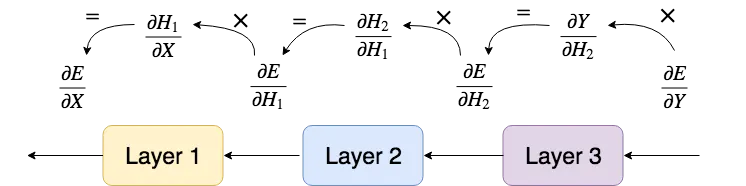
\includegraphics[width=0.7\textwidth]{figures/backpropagation_from_scratch}
	\caption{Graphical example of how back-propagation works.}
	\label{fig:backpropagation_from_scratch}
\end{figure}

\subsection{Fully Connected Layer}
Now let's define and implement the first type of layer: fully connected layer. These are the most basic layers as every input neurons are connected to every output neurons.

The value of each output neuron can be calculated as the following :
\begin{equation}
	y_i = b_j + \sum_i x_i w_{ij}
\end{equation}

With matrices, we can compute this formula for every output neuron in one shot using a dot product: $Y=XW+B$
\emph{Note that I’m not using any activation function yet, that’s because we will implement it in a separate layer.}

As we said, suppose we have a matrix containing the derivative of the error with respect to that layer’s output ($\frac{\partial E}{\partial Y}$). We need:
\begin{itemize}
	\item the derivative of the error with respect to the parameters ($\frac{\partial E}{\partial W}$, $\frac{\partial E}{\partial B}$);
	\item the derivative of the error with respect to the input ($\frac{\partial E}{\partial X}$).
\end{itemize}

Let's calculate $\frac{\partial E}{\partial W}$. This matrix should be the same size as $W$ itself: $i\times j$ where $i$ is the number of input neurons and $j$ the number of output neurons. We need one gradient for every weight and using the chain rule stated earlier, we can write:

\begin{equation}
	\cfrac{\partial E}{\partial w_{ij}} = \cfrac{\partial E}{\partial y_1}\cfrac{\partial y_1}{\partial w_{ij}} + \ldots + \cfrac{\partial E}{\partial y_j}\cfrac{\partial y_j}{\partial w_{ij}} = \cfrac{\partial E}{\partial y_j}x_i 
\end{equation}

Therefore,
\begin{equation}
	\cfrac{\partial E}{\partial W} = X^T\cfrac{\partial E}{\partial Y}
\end{equation}

Same story to calculate $\frac{\partial E}{\partial B}$

\begin{equation}
	\cfrac{\partial E}{\partial b_j} = \cfrac{\partial E}{\partial y_1}\cfrac{\partial y_1}{\partial b_j} + \ldots \cfrac{\partial E}{\partial y_j}\cfrac{\partial y_j}{\partial b_j} = \cfrac{\partial E}{\partial y_j} 
\end{equation}

And conclude that,
\begin{equation}
	\cfrac{\partial E}{\partial B} = \cfrac{\partial E}{\partial Y}
\end{equation}

Now we are left with $\cfrac{\partial E}{\partial X}$ which is very important as it will “act” as $\cfrac{\partial E}{\partial Y}$ for the layer before that one. Again, using the chain rule,

\begin{equation}
	\cfrac{\partial E}{\partial x_i} = \cfrac{\partial E}{\partial y_1}\cfrac{\partial y_1}{\partial x_i} + \ldots \cfrac{\partial E}{\partial y_j}\cfrac{\partial y_j}{\partial x_i} = \cfrac{\partial E}{\partial y_1} w_{i1} + \ldots + \cfrac{\partial E}{\partial y_j} w_{ij} 
\end{equation}

Finally, we can write the whole matrix :
\begin{equation}
	\cfrac{\partial E}{\partial C} = \cfrac{\partial E}{\partial Y}W^T
\end{equation}

\pythoncodenon{code/machine_learning_fclayer.py}

\subsection{Activation Layer}
All the calculation we did until now were completely linear. It's hopeless to learn anything with that kind of model. We need to add non-linearity to the model by applying non-linear functions to the output of some layers. We just need to calculate $\frac{\partial E}{\partial X}$.

We will call $f$ and $f'$ the activation function and its derivative respectively. For a given input $X$, the output is simply the activation function applied to every element of $X$: $Y = f(X)$. 

Given $\frac{\partial E}{\partial Y}$, we want to calculate $\frac{\partial E}{\partial X}$
\begin{equation}
	\cfrac{\partial E}{\partial x_i} = \cfrac{\partial E}{\partial y_i}\cfrac{\partial y_i}{\partial x_i} = \cfrac{\partial E}{\partial y_i} f'(x_i) 
\end{equation}

\pythoncodenon{code/machine_learning_activation.py}

You can also write some activation functions and their derivatives

\pythoncodenon{code/machine_learning_tanh.py}

\subsection{Loss Function}
Until now, for a given layer, we supposed that $\frac{\partial E}{\partial Y}$ was given (by the next layer). But what happens to the last layer ? We simply give it manually, and it depends on how we define the error.


The error of the network, which measures how good or bad the network did for a given input data, is computed by the \emph{loss function}.

Different loss functions will give different error estimates for the same prediction, and thus they have a considerable effect on the performance of any model. Two are the main choices:

\begin{itemize}
	\tightlist
	\item Mean Absolute Error (MAE): the average of the absolute value of the differences between the predictions and true values. It shows how far off we are on average from the correct value;
	\item Mean Squared Error (MSE): the average of the squared differences between the predictions and true values. It instead penalizes larger errors more heavily and is commonly used in regression tasks. Sometimes it is also referred to as \emph{L2-norm}, or squared norm
	\begin{equation}
		L2 = \frac{1}{2}\sum_i (y_i - t_i)^2
	\end{equation} 
\end{itemize}

What we need now, as for every other layer, is to define $\frac{\partial E}{\partial Y}$ (let's assume we are going to use MSE). Except now, we finally reached $E$ !
\begin{equation}
	\cfrac{\partial E}{\partial y_i} = \cfrac{2}{n} (y_i - \tilde{y_i}) 
\end{equation}

\pythoncodenon{code/machine_learning_loss.py}

Either metrics may be appropriate depending on the situation and you can use both for comparison. More information about loss function can be found in~\cite{bib:loss_function}.

\subsection{\texttt{Network} Class}

Finally ee are going to make a \texttt{Network} class to create and run neural networks

\pythoncodenon{code/machine_learning_network.py}

%\subsection{Back-propagation}
%The machine learning process is iterative. Data is fed into the model, then is accuracy is measured through the loss function. Then, with the help of optimization algorithms, the model’s parameters (weights and biases) are varied until the desired outputs are reached.
%
%\emph{Forward-propagation} is the process of pushing inputs through the net. At the end of each epoch, the obtained outputs is compared to the targets to form the errors. In the \emph{back-propagation}~\cite{bib:backpropagation}, the process is reversed and weights and biases are adjusted based on the obtained errors, minimizing the loss, thus improving the accuracy of artificial neural networks.
%Referring to the network in Figure~\ref{fig:training} which contains an input layer, a hidden layer, and an output layer let's describe how it works.
%
%Two inputs, $(x_1, x_2)$, are fed into the network and passed to the hidden nodes, whose ouputs, $a_i$, are finally sent to the output layer which produces the prediction $y_i$. The arrows that connect the nodes represents the weights, e.g. $w^{(l)}_{ij}$ is the weights connecting the $i$th node of the $l$th layer to the $j$th node in the next layer. Finally the predictions are compared to the target outputs $t_i$. 
%
%Without loss of generality, we are going to assume that the used loss function is the L2-norm, and that each node activation function is a \emph{sigmoid} (logistic function)
%
%\begin{equation}
%  \sigma(x) = \frac{1}{1+e^{-x}}
%\end{equation} 
%and its derivative (will be useful later on)
%\begin{equation}
%  \frac{\partial\sigma(x)}{\partial x} = \sigma(x)(1-\sigma(x))
%  \label{eq:sigmoid_derivative}
%\end{equation} 
%
%\subsubsection{Back-propagation for the Output Layer}
%The idea of back-propagation is to compute the gradient of the loss function concerning the weights and biases of each neuron in the network. Then, we use the gradients obtained to update the parameters such that the loss computed at the new value is less than the loss at the current value. The loss decreases by iteratively adjusting the weights and biases based on the obtained gradients, and the network gradually learns to make better predictions.
%
%The updates are directly related to the partial derivatives of the loss and to the errors (the differences between targets and outputs). The update rule can be written as
%\begin{equation}
%  w \leftarrow w - \eta\nabla_w L(w)
%\end{equation}
%where $\eta$ is the algorithm's \emph{learning rate}.
%
%To compute the right hand side of the previous expression we can use the chain rule. Considering for simplicity just one weight 
%\begin{equation}
%  \frac{\partial L}{\partial w^{(2)}_{ij}} = \frac{\partial L}{\partial y_j}\frac{\partial y_j}{\partial a^{(2)}_j}\frac{\partial a^{(2)}_j}{\partial w^{(2)}_{ij}}
%\label{eq:backprop_output}
%\end{equation}
%where $i$ corresponds to the hidden layer, $j$ corresponds to the output layer, and $a^{(2)}$ represents the input to the activation function (the linear combination of the neuron input) of a node in the second layer.
%The first the three terms is the loss derivative, since we are using the L2-norm it becomes
%\begin{equation}
%  \frac{\partial L}{\partial y_j} = (y_j - t_j)
%\end{equation}
%The second one is the sigmoid derivative (see Eq.~\ref{eq:sigmoid_derivative}):
%\begin{equation}
%  \frac{\partial y_j}{\partial a^{(2)}_j} = \sigma(a^{(2)}_j)(1-\sigma(a^{(2)}_j)) = y_j(1 - y_j)
%\end{equation}
%where the last step is due to the fact we are considering the output layer.
%Finally, the third one is the derivative of $a_j$ (i.e. the input value of the activation function) which equals
%\begin{equation}
%  \frac{\partial a^{(2)}_j}{\partial w^{(2)}_{ij}} = h_i
%\end{equation}
%where $h_i$ is the output of the $i$th node of the hidden layer.
%
%Replacing the partial derivatives into Eq.~\ref{eq:backprop_output} above, we get
%\begin{equation}
%  \frac{\partial L}{\partial w^{(2)}_{ij}} = (y_j - t_j) y_j(1 - y_j) h_i
%\end{equation}
%
%This is the update rule for a single weight for the output layer in our example network.
%
%\subsubsection{Back-propagation for a Hidden Layer}
%Similarly to the back-propagation of the output layer $\frac{\partial L}{\partial w^{(1)}_{ij}}$, the update rule for a single weight in a hidden layer, is given by Eq.~\ref{eq:backprop_output}, and again it can be computed following the chain rule.
%
%The calculation of the last two terms of the right hand side are the same as in the output layer case, but the calculation of the first component is more complex.
%The problem is that we don’t have targets for the hidden layers’ outputs, so we can’t calculate the errors as we did for the output layers.
%Instead, we solve this issue by tracing the contribution of each neuron (hidden or not) to the outputs’ errors. Let’s illustrate this with the following back-propagation example.
%
%The weight $w^{(1)}_{11}$ contributes to $h_1$. But $h_1$ is connected to the weights $w^{(2)}_{11}$ and $w^{(2)}_{12}$, contributing to two outputs. This means we can trace the contribution of $w^{(1)}_{11}$ to two outputs ($y_1$ and $y_2$) and errors ($e_1$ and $e_2$).
%
%We take the errors and back-propagate them through the net using the $w^{(2)}_{1j}$ weights. This allows us to measure the contribution of the hidden layers to the respective errors and use it to update the $w^{(1)}$ weights.
%
%Let’s take the solution for weight $w^{(1)}_{11}$ as an example:
%\begin{align}
%	\frac{\partial L}{\partial h_1} &= \frac{\partial L}{\partial y_1}\frac{\partial y_1}{\partial a^{(2)}_1}\frac{\partial a^{(2)}_1}{\partial h_1} + \frac{\partial L}{\partial y_2}\frac{\partial y_2}{\partial a^{(2)}_2}\frac{\partial a^{(2)}_2}{\partial h_1} \\ 
%	& = (y_1 - t_1)y_1(1-y_1)w^{(2)}_{11} + (y_2 - t_2)y_2(1-y_2)w^{(2)}_{12}
%\end{align}
%
%Now, we can calculate $\frac{\partial L}{\partial w^{(1)}_{11}}$ %, which was the only missing part of the update rule for the hidden layer.
%whose final expression is
%\begin{equation}
%  \frac{\partial L}{\partial w^{(1)}_{11}} = [(y_1-t_1)y_1(1-y_1)w^{(2)}_{11}+(y_2-t_2)y_2(1-y_2)w^{(2)}_{12}]h_1(1-h_1)x_1	
%\end{equation}
%The generalized form of this equation is:
%\begin{equation}
%  \frac{\partial L}{\partial w^{(l)}_{ij}} = \sum_k(y_k-t_k)y_k(1-y_k)w^{(l+1)}_{ij}h_j(1-h_j)x_i
%\end{equation}
%In our programs the \emph{optimization function} that will be used is \emph{Adam}.

